Not every system can be studied in discrete time jumps. When time becomes a continuous variable, dynamical systems have to be represented using equations that work for any possible time interval. The mathematical tool of choice in these cases are differential equations.


A differential equation is an equality involving one or more unknowns ($x$, $y$, $z$,\dots) and their derivatives ($x'$, $y'$, $z'$,\dots). Since our unknowns have derivatives, they are not just numbers like in regular -- a.k.a. algebraic -- equations. Our unknowns are functions or, more accurately, families of functions. In the case of dynamic systems, all our state variables will be functions of time, we can make this explicit by writing them as $x(t)$, $y(t)$, $z(t)$,\dots thus sacrificing brevity for the sake of clarity. This time dependency is not always made explicit since it is known from the context so we will often define a variable as $x$ instead of $x(t)$ just to keep the notation simple.
Now that we introduce time $t$ as a continuous variable, we cannot think of the evolution of our variables as jumps from one generation to another. Whenever we observe a change, we have to keep in mind that it happens within a time interval $(t_0, t_f)$. The amount of time along the interval will be denoted as the increment $\Delta t = t_f - t_0$, and the corresponding increment in other variables will follow the same notation $\Delta x, \Delta y, \Delta z, \dots$.

\section{Derivatives}

We will concern ourselves with differential equations involving functions of time, so given a dependent variable $x(t)$, we will refer to its derivative with respect to time using any of the three notations: 

\begin{equation*}
	x' = \dot{x} = \frac{dx}{dt}  
\end{equation*}

As a reminder from high school mathematics, $dx$ and $dt$ represent very small increments of $x$ and $t$ respectively, so for very short time intervals:

\begin{equation*}
\frac{\Delta x}{\Delta t}   \approxeq \frac{dx}{dt}  
\end{equation*}

So when we write the differential equation:

\begin{equation}
	\frac{dx}{dt}  = 3
\label{simplestode}
\end{equation}

What we are saying is that for every time unit that passes, our variable $x$ increases by 3 units. Obviously, derivatives have units. For instance, if the equation above was describing infected individuals in a population surveyed every year, the equation would be saying: there will be an increase of 3 individuals per year. In general, the units of $\frac{dx}{dt}$ are units of $x$ divided by units of $t$.

Even when we cannot solve a differential equation, we can still test possible solutions. For instance, we may propose  that $x(t) = 3\, t + 7$ is a solution for equation \ref{simplestode}. To test that hypothesis we can apply the usual derivation rules and find that, indeed, $x' = 3$, so we have found a solution to our equation. If we keep trying solutions like this, we will soon find that replacing $7$ with any other number will still result in new solutions. that is why we can write: 

\begin{equation}
	x(t) = 3\, t + C
	\label{simplestode_sol}
\end{equation}

As the \textbf{general solution} of the equation. for every possible numerical value of $C$, we will obtain a \textbf{particular solution}. The general solution of a differential equation represents a family of functions and it is normally of interest to mathematicians. Scientists and engineers are normally interested in making predictions for real life situations, which normally means finding a specific particular solution. In the case of equation \ref{simplestode}, our question may be: ``How many infected individuals will we have in thrree years if we start with $25$ infected?'' we can find our solution by substituting the  initial value $x(0)=25$ in equation \ref{simplestode_sol} when $t=0$

\begin{equation*}
	3\, 0 + C = 25
\end{equation*}

So our particular solution is  $x(t) = 3\, t + 25$. Particular solutions can also be calculated by computer simulations, even in cases when no general solution can be found. In fact, finding general solutions for a differential equation is a very challenging problem and most equations have no known general solution that can be expressed by a mathematical formula.

Among all differential equations, we will be interested in the simpler type. Ordinary differential equations (ODEs) are those that do not involve partial derivatives. Moreover, we will start with linear equations.

\section{Linear equations}

Linear equations are those where different unknowns and their derivatives are only combined linearly. Some examples of linear equations are:

\begin{align}
	\frac{dx}{dt} \: = \: &  a \, x	\nonumber\\
	\frac{dx}{dt} + \frac{dy}{dt}\: = \: &  0 \nonumber\\
	\frac{dx}{dt} \: = \: &  a \, x + b \, y \nonumber
\end{align}

while the following equations are not linear:

\begin{align}
	\frac{dx}{dt} \: = \: &  x^2	\nonumber\\
	\frac{dx}{dt} + \frac{dy}{dt}\: = \: &  x \, y \nonumber\\
	\frac{dx}{dt} \: = \: &  \sin x \nonumber
\end{align}

Keep in mind that the linearity requirement only applies to the unknowns and not to the independent variable, time. The following equations are all linear


\begin{align}
	\frac{dx}{dt} \: = \: &  t^2 \, x	\nonumber\\
	\frac{dx}{dt} + \frac{dy}{dt}\: = \: &  \sin t \nonumber\\
	\frac{dx}{dt} \: = \: &  t \, x + t^2 \, y \nonumber
\end{align}

In these equations, the coefficients that multiply our unknowns just happen to be functions of time. A linear equation can have coefficients that depend on time and also have time-dependent independent terms. In general, we will not concern ourselves with such systems.



Solving differential equations is very challenging, that's why we will try to avoid it whenever possible. In fact, we are only going to solve one differential equation during the whole course. We will solve it in two versions: with one variable and with several variables.

\subsection{Solving the linear equation with one variable}

Lets start with the simplest possible case, which also happens to describe a fundamental biological process: exponential growth.

\begin{equation}
	\label{odexp}
	\frac{dx}{dt} = \mu \, x 
\end{equation}

This can be read as: ``the rate of increase of a population $x$ is directly proportional to its own size.'' This equation is easy to solve because we can separate the variables:


\begin{equation}
	\frac{dx}{x} = \mu \, dt \nonumber
\end{equation}

and integrate

\begin{equation}
	\int \frac{dx}{x} = \mu \, \int  dt \nonumber
\end{equation}

\begin{equation}
	\ln{x} = \mu \, t + C \nonumber
\end{equation}

Since $C$ is an arbitrary constant, we can define it in terms of another constant $C= \ln{k}$ so:

\begin{equation}
	\ln{x} - \ln{k}  = \mu \, t  \nonumber
\end{equation}

Applying the well known properties of logarithms listed in appendix \ref{logprop}

\begin{equation}
	\ln{\frac{x}{k}}   = \mu \, t \nonumber
\end{equation}

exponentiating both sides and rearranging

\begin{equation}
	x   = k \, e^{\mu \, t} \nonumber
\end{equation}

This is the \emph{general solution} of the differential equation but, as stated before, we are not normally interested in general solutions. General solutions are for mathematicians. We want the particular solution that fits some \emph{initial condition} when $t=0$,  often written $x(0)$ or $x_0$. For instance, we have a bacterial culture that starts with an optical density of 0.01. How do we find the right value for k?


\begin{equation}
x(0) = 0.01 \Rightarrow	 k \, e^{\mu \, 0} = 0.01 \Rightarrow	k=0.01 \nonumber
\end{equation}

In general, we use the solution to the exponential equation as:

\begin{equation}
	x   = x_0 \, e^{\mu \, t} \nonumber
\end{equation}

\paragraph{Exercise:} Can you find an expression for the duplication time in exponential growth?

\subsection{Solving the linear equation with several variables}


Our simple linear equation can also have more that one variable:

\begin{align}
	\label{odenvar}
	\frac{dx_1}{dt} =& a_{1,1} \, x_1 + a_{1,2} \, x_2 \nonumber\\
	\frac{dx_2}{dt} =& a_{2,1} \, x_1 + a_{2,2} \, x_2
\end{align}

As seen in the previous chapter, vectors and matrices are extremely useful when dealing with several variables.

\begin{equation}
	\frac{d}{dt} \begin{pmatrix} x_1\\ x_2 \end{pmatrix} = \begin{pmatrix} a_{1,1} & a_{1,2}\\ a_{2,1} & a_{2,2} \end{pmatrix} \begin{pmatrix} x_1\\ x_2 \end{pmatrix} \nonumber
\end{equation}

Thus, we can write any equation with n variables as:

\begin{equation}
	\label{odenvar_mat}
	\frac{d\mathbf{x}}{dt}  = \mathbf{A} \, \mathbf{x}
\end{equation}

Since the solution of the equation for one variable was an exponential, lets make the hypothesis that an exponential can also be a solution for this case. We assume

\begin{equation}
	\mathbf{x}= \mathbf{v} \, e^{\lambda \, t} \nonumber
\end{equation}

But $\mathbf{x}$ is a vector now, so we multiply our exponential times a  vector of constants $\mathbf{v}$ to be sure that the result is a vector as well. We can test if this is a valid solution by substituting it into the equation, which gives:

\begin{equation}
	\frac{d}{dt} \left( \mathbf{v} \, e^{\lambda \, t} \right)  = \mathbf{A} \, \mathbf{v} \, e^{\lambda \, t}  \nonumber
\end{equation}

On the left hand side, the vector of  constants can be taken out of the derivative so:

\begin{equation}
	\mathbf{v} \, \frac{d}{dt} \left(  e^{\lambda \, t} \right)  = \mathbf{A} \, \mathbf{v} \, e^{\lambda \, t}  \nonumber
\end{equation}
 
 and on the right hand side
 
 \begin{equation}
 	\mathbf{v}   \lambda \, e^{\lambda \, t}   = \mathbf{A} \, \mathbf{v} \, e^{\lambda \, t} \nonumber
 \end{equation}
 
canceling out the exponentials:

\begin{equation}
\mathbf{A} \, \mathbf{v}  = \lambda  \,	\mathbf{v}   
\end{equation}
 
So $\mathbf{x}=\mathbf{v} \, e^{\lambda \, t}$ will be a solution of the equation as long as $\lambda$ and $\mathbf{v}$ satisfy the equation above, which we had already seen before in equation (\ref{eigendefinition}). In other works, the solution will only be correct if the chosen vector $\mathbf{v}$ is an eigenvector of $\mathbf{A}$ and the exponent $\lambda$ is the corresponding eigenvalue.

So to find the solution of any linear equation of this type, regardless of the number of variables, we just have to calculate the eigenvalues and eigenvectors of matrix $\mathbf{A}$.

\section{Calculating eigenvectors and eigenvalues}
If we rearrange terms in the definition of eigenvectors and eigenvalues:

\begin{equation}
	\mathbf{A} \, \mathbf{v}  - \mathbf{I} \, \lambda  \,	\mathbf{v}   = 0 \nonumber
\end{equation}

note we have multiplied lambda by the identity matrix $\mathbf{I}$. This is a matrix of zeros everywhere except its main diagonal, which is occupied by ones. The identity matrix plays the same role as number one among scalars, it does not alter the matrices or vectors it multiplies.Introducing the identity matrix keeps the equation unchanged because  $\mathbf{I} \, \lambda  \,	\mathbf{v}  =\lambda  \,	\mathbf{v} $.  The reason why we need it, is that now we can factor $\mathbf{v}$ out 

\begin{equation}
	\label{solve4eigenvec}
	\left( \mathbf{A}   - \mathbf{I} \, \lambda     \right) \, \mathbf{v} =  0  
\end{equation}

Without the identity matrix, the parenthesis will have a scalar subtracted from a matrix, which cannot be done. In a two-variable system, equation \ref{solve4eigenvec} would look like this:

\begin{equation}
\begin{pmatrix} a_{1,1} - \lambda & a_{1,2}\\ a_{2,1} & a_{2,2}  - \lambda \end{pmatrix} \begin{pmatrix} v_1\\ v_2 \end{pmatrix} =  \begin{pmatrix} 0\\ 0 \end{pmatrix}\nonumber
\end{equation}

This is an homogeneous system of equations with the components of $\mathbf{v}$ as unknowns. For the system to have a solution other than the trivial, $\mathbf{v}=\mathbf{0}$, the determinant of the parenthesis must satisfy:

\begin{equation}
	\label{solve4eigenval}
	\left| \mathbf{A}   - \mathbf{I} \, \lambda     \right|  =  0  
\end{equation}

The eigenvector is no longer part of the equation, so we can now solve for lambda. The expansion of this determinant results in a $n-th$ degree equation in terms of lambda known as the characteristic polynomial of the system.

\begin{equation}
c_n \, \lambda^n +c_{n-1} \, \lambda^{n-1}  + \dots  + c_1 \, \lambda + c_0 = 0 \nonumber
\end{equation}

Solving this provides the values of all the eigenvalues of the matrix. By substituting each eigenvalue in equation \ref{solve4eigenvec}, we can obtain the corresponding eigenvectors.

\section{The eigenvalues of a differential equation} 

\subsection{Real eigenvalues}

Lets take the matrix
\begin{equation}
	\mathbf{A}  = \begin{pmatrix} -1 & -4\\ -3 & -2\end{pmatrix} \nonumber
\end{equation}

If we transform  vector (4,-3)

\begin{equation}
	\begin{pmatrix} -1 & -4\\ -3 & -2\end{pmatrix} \,  \begin{pmatrix} 4\\ -3\end{pmatrix}=\begin{pmatrix} 8 \\ -6\end{pmatrix}\nonumber
\end{equation}

we obtain a stretched version of itself with double length. If we now transformed $(8,-6)$ using the matrix, we would obtain $(16,-12)$, which is again the same vector multiplied by two. So (4,-3) is an eigenvector of $\mathbf{A}$ and the corresponding eigenvalue is $\lambda=2$. 

But how can we find out the eigenvectors and eigenvalues of a matrix other than by trial and error? First we get the eigenvalues using equation \ref{solve4eigenval}:

\begin{equation}
  \left|\begin{matrix} -1-\lambda & -4\\ -3 & -2-\lambda\end{matrix} \right| = 0 \nonumber
\end{equation}

we get the characteristic polynomial

\begin{equation}
	\lambda^2  +3 \,  \lambda  - 10 = 0 \nonumber
\end{equation}

A primary school problem we can solve:

\begin{equation}
	\lambda= \frac{-3 \pm \sqrt{9+40}}{2} \nonumber
\end{equation}

with two solutions $\lambda_1=-5$ and $\lambda_2=2$. We have already seen that the eigenvector $\mathbf{v_2}$ for $\lambda_2$ is (4,-3). Can we find the other one? We can go back to equation (\ref{eigendefinition}) or use the already factored out version in equation  (\ref{solve4eigenvec})

\begin{equation}
\begin{pmatrix} -1-\lambda & -4\\ -3 & -2-\lambda\end{pmatrix} \, \begin{pmatrix} v_x \\  v_y\end{pmatrix} = 0 \nonumber
\end{equation}

For the case $\lambda = -5$:

\begin{equation}
	\begin{pmatrix} 4 & -4\\ -3 & 3\end{pmatrix} \, \begin{pmatrix} v_x \\  v_y\end{pmatrix} = 0 \nonumber
\end{equation}

\begin{align*}
	4 \, v_x - 4 \, v_y =& 0 \nonumber\\
	-3 \, v_x + 3 \, v_y =& 0 \nonumber
\end{align*}

Which is the same equation twice, so there is no unique solution. This shows a very important property of eigenvectors: they are never unique. It is easy to see that whenever  $v_x=v_y$ both equations cancel out. If choose $v_x=1$, then our eigenvector will be $\mathbf{v}=\left( 1,1 \right)$. We could just as well have chosen a different $v_x$ and obtain vectors $\left( 2,2 \right)$, $\left( 3,3 \right)$ , etc.


\subsection{Complex eigenvalues}

Now lets analyze another matrix 

\begin{equation}
	\mathbf{A}  = \begin{pmatrix} 0 & -1\\ 1 & 0\end{pmatrix}  \nonumber
\end{equation}

Characteristic polynomial

\begin{equation}
	\lambda^2 + 1 = 0 \nonumber
\end{equation}

The solutions to this equation are imaginary $\lambda_1 = i$ and $\lambda_1 = -i$.

Complex eigenvalues always come in conjugate pairs: $\lambda_1 = a + b\, i$,  $\lambda_2 = a - b\, i$. As we will see in the next section, the real parts of a complex eigenvalue determine the stability, while the existence of imaginary parts involves the existence of oscillations. Note that imaginary eigenvalues can only appear for systems with two or more variables. This means that for a system to oscillate, it must have at least two variables.


\section{General solutions for linear equations}

So putting together all the eigenvectors of the system and the corresponding eigenvalues, we get the general solution for our equation with n variables:


\begin{equation}
	\label{odenvar_mat_sol}
	\mathbf{x}= c_1 \, \mathbf{v_1} \, e^{\lambda_1 \, t} + c_2 \, \mathbf{v_2} \, e^{\lambda_2 \, t} +  \dots + c_n \, \mathbf{v_n} \, e^{\lambda_n \, t} 
\end{equation}

Where $c_1 \dots c_n$  are arbitrary constants, the ones that can be used to adjust initial values. Each vector $\mathbf{v_i}$ and its corresponding constant $\lambda_i$ are called eigenvector and eigenvalue respectively.
\paragraph{Example:} lets assume our system has eigenvectors $\mathbf{v_1}=\begin{pmatrix} 1 \\ 1 \end{pmatrix}$ and
	$\mathbf{v_2}=\begin{pmatrix} 1 \\ -1 \end{pmatrix}$. If the eigenvalues are $\lambda_1=2$ and $\lambda_2=1$, the general solution will be:
\begin{equation}
	\mathbf{x}= c_1 \, \begin{pmatrix} 1 \\ 1 \end{pmatrix} \, e^{2 \, t} + c_2 \, \begin{pmatrix} 1 \\ -1 \end{pmatrix} \, e^{ t} 
\end{equation}

To get the particular solution for a system with initial value $\mathbf{x_0}=\begin{pmatrix} 0 \\ 2 \end{pmatrix}$, we have to find the values of the arbitrary constants such that for $t=0$:

\begin{equation}
	\begin{pmatrix} 0 \\ 2 \end{pmatrix}= c_1 \, \begin{pmatrix} 1 \\ 1 \end{pmatrix} \, e^{0} + c_2 \, \begin{pmatrix} 1 \\ -1 \end{pmatrix} \, e^{0} 
\end{equation}

which means $c_1=1$,$c_2=-1$. And our particular solution will be:

\begin{equation}
	\mathbf{x(t)}=   \begin{pmatrix} 1 \\ 1 \end{pmatrix} \, e^{2 \, t} +  \begin{pmatrix} -1 \\ 1 \end{pmatrix} \, e^{t} 
\end{equation}

Note that any positive eigenvalue will result in a positive exponential that will keep increasing with time. For this reason, any system with one or more positive eigenvalues, will have some variables increasing to infinity, and will be said to be unstable. On the other hand, in a system where all eigenvalues are negative, all variables will tend to zero, so they will be considered stable.


When the eigenvalues (and eigenvectors) are complex, the solutions described above will be complex. But we are not interested in complex solutions, since all our models have real variables. In fact, as happened with Leslie matrices, complex eigenvalues cause oscillations in the real solutions of the system, lets see a combination of complex exponentials:

\begin{equation}
	x_1= c_1 e^{\left(  a + b\, i\right) \, t} + c_2 \,  e^{\left(  a + b\, i\right)\, t} = 
	c_1  \, e^{a \, t} \, e^{ i \, b \, t} + c_2 \,  e^{a \, t} \, e^{-i \, b \, t} 
	\nonumber
\end{equation}

factoring out the real exponential

\begin{equation}
x_1= e^{a \, t} \,  \left( c_1  \, e^{ i \, b \, t} + c_2 \,  e^{-i \, b \, t}\right) \nonumber
\end{equation}

Using Euler's formula:

\begin{equation}
	\label{euler}
	e^{i \theta} = cos \theta + i \, \sin \theta 
\end{equation}

\begin{equation}
	x_1= e^{a \, t} \,  \left( c_1  \, \left(  \cos{ b \, t} + i \, \sin{ b \, t} \right)+ c_2 \, \left( \cos{- b \, t} + i \, \sin{- b \, t} \right) \right) \nonumber
\end{equation}

\begin{figure}
\begin{center}
	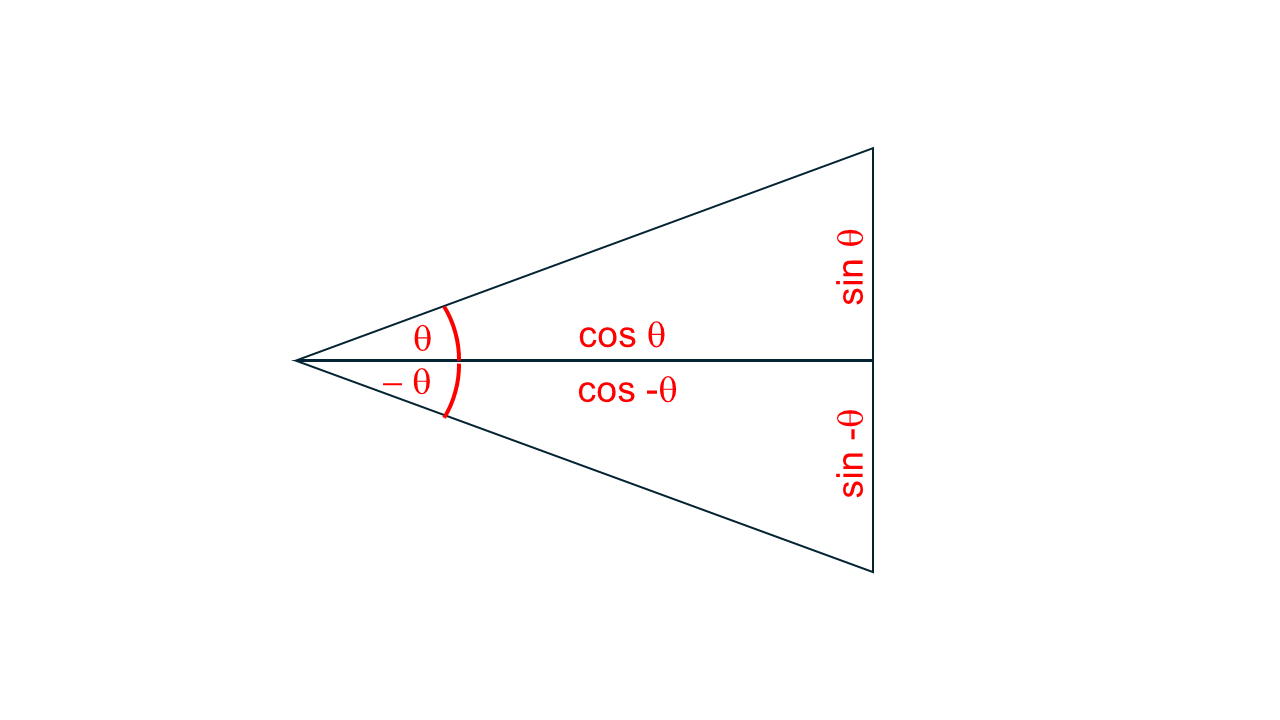
\includegraphics[width=\textwidth]{trigo}
\end{center}
\caption{Some basic trigonometric relations.}
\label{fig:trigo}
\end{figure}

As can be seen in  figure \ref{fig:trigo}, $- \sin{b \, t}=\sin{- b \, t}$ and $\cos{b \, t}=\cos{ - b \, t}$ so we can rearrange terms:

\begin{equation}
	x_1= e^{a \, t} \,  \left( c_1  \, \left(  \cos{ b \, t} + i \, \sin{ b \, t} \right)+ c_2 \, \left( \cos{ b \, t} - i \, \sin{ b \, t} \right) \right) \nonumber
\end{equation}


\begin{equation}
	x_1=   \left( c_1+c_2\right) \, e^{a \, t} \, \cos{ b \, t}  + i \, \,\left( c_1-c_2 \right) \,e^{a \, t} \,   \sin{ b \, t}   \nonumber
\end{equation}

Note that this solution has the form $x_1(t) = u(t) + i \, v(t)$ where both $u(t)$ and $v(t)$ are real functions. Moreover, these functions are linearly independent so a combination of both will be a proper general solution. By defining new arbitrary constants, we will get the general solution that includes al possible real solutions of the equation:

\begin{equation}
	x_1=   e^{a \, t} \,  \left(  A  \, \cos{ b \, t}  +  B  \,   \sin{ b \, t}  \right) \nonumber
\end{equation}

So the real part of our solutions will be the product of an exponential and an oscillatory function. Moreover, the exponential depends only on the real part of the eigenvalue, $\operatorname{Re}(\lambda) = a$, while the oscillations depend on its imaginary part,  $\operatorname{Im}(\lambda) =b$ (see figure \ref{fig:cmplxeigen}). 

\begin{figure}
	\begin{center}
		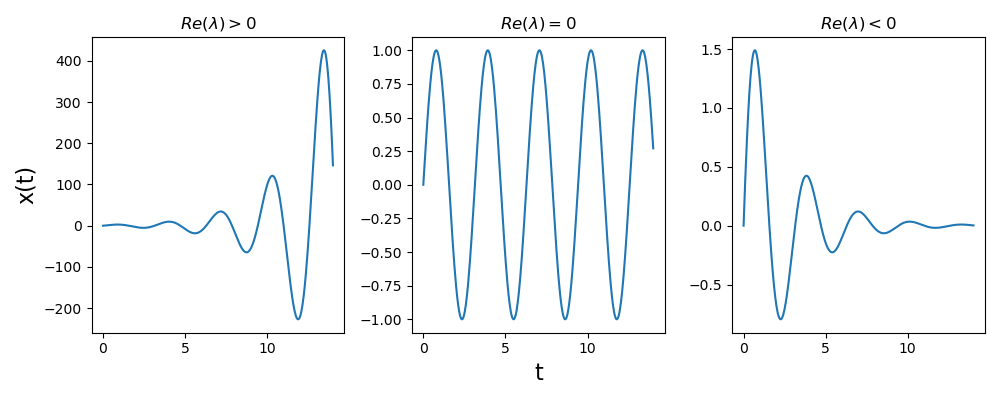
\includegraphics[width=\textwidth]{complex_eigen}
	\end{center}
	\caption{Overal behavior of solutions when eigenvalues are complex. The sign of $\operatorname{Re}(\lambda)$ determines stability and $\operatorname{Im}(\lambda)$ governs oscillations}
	\label{fig:cmplxeigen}
\end{figure}


\FloatBarrier

\subsection{Differential equations of higher order}

The following differential equation:

\begin{equation}
	 \frac{d^2x}{dt^2} = \frac{k}{m} \, x - g \nonumber
\end{equation}

is called a second order differential equation because it contains a second derivative. This equation can lead to oscillations, even though, we just said only systems with two variables can show this behavior. The reason for that is that any  differential equation of order $n$ can be written as a first order differential equation with n variables. If we add the variable $y(t)$ as the derivative of $x(t)$ to the equation above, it becomes:

\begin{align}
	\frac{dx}{dt} =& \: y \nonumber \\
	\frac{dy}{dt} =& \: \frac{k}{m} \, x - g \nonumber
\end{align}

So any differential equation of order $n$ can be considered a first order differential equation with $n$ variables.

\subsection{Plotting solutions}

The particular solutions of a differential equation can be plotted as each variable being a function of time as shown in figure \ref{fig:cmplxeigen}, but there are alternative representations. A frequently used plot is the phase space like the one shown in figure \ref{fig:phase_plane}. In this plot, the state variables of the system are used as axes. Since time is not explicitly included in the plot, the lines showing the evolution of the system have arrows that indicate the direction in which the system moves as time goes by. In a plot like this, several particular solutions can be shown at the same time, the line representing each solution is called an orbit. 
\begin{figure}
	\begin{center}
		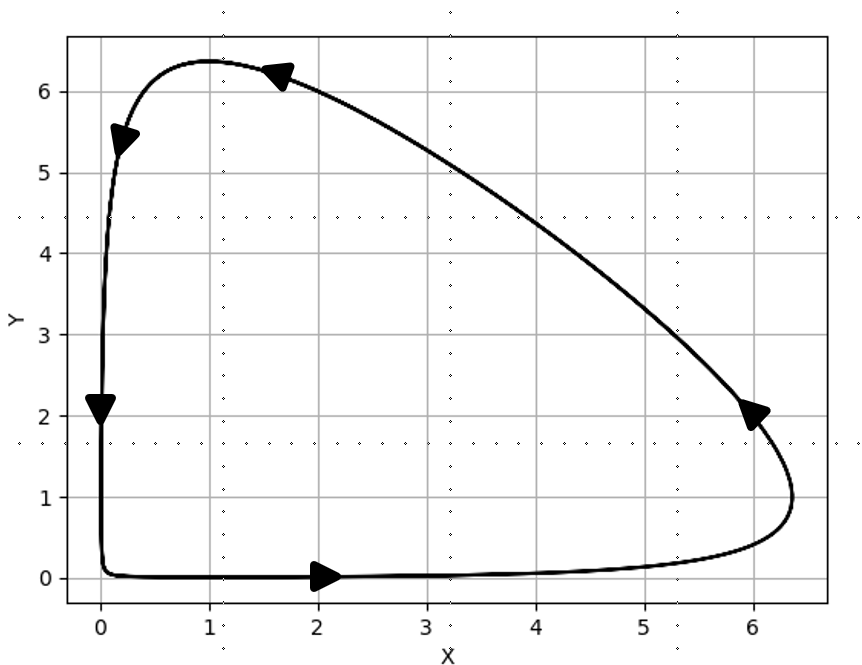
\includegraphics[width=0.7\textwidth]{phase_plane}
	\end{center}
	\caption{Phase plane representation of a particular solution of a two variable oscillatory system.}
	\label{fig:phase_plane}
\end{figure}

\section{Non-linear systems}

Unlike linear equations, non-linear equations rarely have analytic solutions. Fortunately, we can extract a lot of information from a differential equation without solving it. This is so because we are often not interested in every detail about its dynamics but rather on its long term behavior.

\subsection{Steady states}

The first step to analyze non-linear systems is to find out their steady states. for a given non-linear system:

\begin{equation}
	\label{odegeneral}
	\frac{d\mathbf{x}}{dt} = \mathbf{f}(\mathbf{x})
\end{equation}

we can calculate its steady states as those values $\mathbf{x}= \mathbf{x_0}$ such that:

\begin{equation}
	\label{stst}
	\mathbf{f}(\mathbf{x_0}) = 0
\end{equation}

Steady states are important because once the system reaches it, it will remain in it as long as it is not perturbed.

\paragraph{Example:} Lets take another growth equation:

\begin{equation}
	\label{odgrowth}
	\frac{dx}{dt} = \mu(x) \, x 
\end{equation}

Unlike exponential growth, where $\mu$ is constant, this more general form makes the growth rate dependent on the size of the population. This model is more realistic as resources are expected to become scarce once the population density becomes too high. A particular case is that of logistic growth, where $\mu(x) = \mu_{m} (1 - x / K)$. Our equation becomes

\begin{equation}
	\label{logistic}
	\frac{dx}{dt} = \mu_{m} \left(1 - \frac{x}{K} \right) \, x 
\end{equation}

The steady state condition will be:

\begin{equation}
 \mu_{m} \left(1 - \frac{x}{K} \right) \, x = 0
\end{equation}

This can happen in two different ways. Either $x=0$, just like happened for exponential growth, or $x=K$.

\begin{figure}
	\begin{center}
		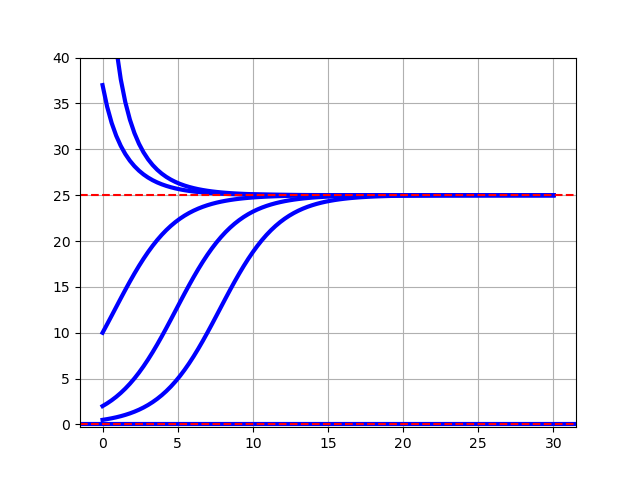
\includegraphics[width=0.8\textwidth]{logisticall}
	\end{center}
	\caption{Logistic growth model with $K=25$, the two steady states $x=0$ and $x=25$ are marked with red dashed lines. It can clearly be seen that the system tends to move away from one steady state and towards the other.}
	\label{fig:logisticall}
\end{figure}

\subsection{Stability}

Figure \ref{fig:logisticall} shows how the behavior of the logistic equation is dictated by its two steady states. The system tends to move away from $x=0$, which is therefore called an \emph{unstable steady state} or \emph{repulsor} and towards $x=K$, which is a \emph{stable steady state} or \emph{attractor}. But how do we know whether a steady state is stable?

A steady state is said to be stable when the system tends to return to it after being moved away from it. In other words, lets assume a system has a steady state at $x=x_0$ and we move the system to another, nearby state $x_0+\delta x$. $\delta x$ is a small number and we call it a perturbation. if we define our variable as a composition of the steady state and a time varying perturbation: $x(t) = x_0 + \delta x(t)$, the system can be said to be stable if $\delta x \rightarrow 0$ as $t \rightarrow \infty$. Conversely, we say the system is unstable if $\delta x \rightarrow \infty$ as $t \rightarrow \infty$.  But how can we predict the behavior of $\delta x$? since we can only solve linear systems, we will have to turn equation \ref{odegeneral} into a linear equation \dots

\subsection{Linearization}

Making the change of variable $x(t) = x_0 + \delta x(t)$ in equation \ref{odegeneral},

\begin{equation}
	\frac{d}{dt} \left( x_0 + \delta x(t) \right) = f(x_0 + \delta x(t)) \nonumber
\end{equation}

The left hand side is the  derivative of a sum and can be rewritten as the sum of derivatives. Moreover, since $\delta x$ is small by definition, we can approximate this as a linear system as shown in equation \ref{TaylorLin} in the appendix.

\begin{equation}
	 \frac{dx_0}{dt} + \frac{d}{dt}\delta x(t)  = f(x_0) +\left|\frac{df}{dx}\right|_0 \, \delta x(t)) \nonumber
\end{equation}

$x_0$ is constant, so $\frac{dx_0}{dt}=0$ and $f(x_0)=0$ by the definition of steady state. This leaves the system 

\begin{equation}
	\label{svl}
	\frac{d}{dt}\delta x(t)  =  \left|\frac{df}{dx}\right|_{x=x_0} \,  \delta x(t)) 
\end{equation}

Equation \ref{svl} is called variational linearized system and it is easily to solve. If $\left|\frac{df}{dx}\right|_0 < 0$ then $\delta x \rightarrow 0$ and the steady state is stable. If $\left|\frac{df}{dx}\right|_0 > 0$, $\delta x \rightarrow \infty$ and the system is unstable.

\paragraph{Example:} In the logistic equation:

\begin{equation}
\frac{df}{dx} = \mu_{m} \left( 1-\frac{2 x}{K}\right) \nonumber
\end{equation}

 So for the steady state $x=0$, $\left|\frac{df}{dx}\right|_0 = \mu_m$ and the l.v.s. is:
 
 \begin{equation}
 	\frac{d}{dt}\delta x(t)  = \mu_m \,  \delta x(t))  \nonumber
 \end{equation}
The solution to this equation is a positive exponential so the perturbation $\delta x(t)$ will be amplified with time. This means the steady state is unstable.

and for the steady state $x=K$,  $\left|\frac{df}{dx}\right|_0 = - \mu_m$:

 \begin{equation}
	\frac{d}{dt}\delta x(t)  = -  \mu_m \,  \delta x(t))  \nonumber
\end{equation}Since the solution of this equation is a negative exponential, any perturbation will fade with time and the steady state is stable.

For systems with more variables:

\begin{align}
	\frac{dx}{dt}=&f_x(x,y)  \nonumber\\
	\frac{dy}{dt}=&f_y(x,y)  \nonumber
\end{align}

the l.v.s. looks like this

 \begin{equation}
 	\label{fig:svlnvar}
	\frac{d}{dt} \begin{pmatrix} \delta x\\ \delta y \end{pmatrix}= \begin{pmatrix} \frac{\partial f_x}{\partial x} & \frac{\partial f_x}{\partial y}\\ \frac{\partial f_y}{\partial x} & \frac{\partial f_y}{\partial y} \end{pmatrix} \, \begin{pmatrix} \delta x\\ \delta y \end{pmatrix}
\end{equation}

Again, the Jacobian matrix contains the partial derivatives evaluated at the steady state, so it is a matrix of constants.

\paragraph{Example:} The chemical signaling system in figure \ref{fig:signalpathd} has two components $X$ and $R$ which responds to an input signal $S$:

\begin{align}
	\frac{dR}{dt} =&\: k_1 \, S - k_2 \, X \, R  \nonumber\\
	\frac{dX}{dt} =&\: k_3 \, S - k_4 \, X  \nonumber
\end{align}

\begin{figure}
	\begin{center}
		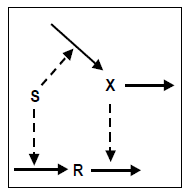
\includegraphics[width=0.3\textwidth]{signalpathd}
	\end{center}
	\caption{A signaling pathway with input $S$ and output $R$. }
	\label{fig:signalpathd}
\end{figure}

The system has a steady state at:

\begin{align}
	R =&\: \frac{k_1 k_4}{k_2 k_3}  \nonumber\\
	X =&\: \frac{k_3}{k_4}S \nonumber
\end{align}

and the jacobian matrix:

\begin{equation}
\mathbf{J} =	 \begin{pmatrix} - k_2 \, X &  - k_2 \, R \\   0  & -k_4 	\end{pmatrix} \nonumber
\end{equation}

Since we are interested in a particular steady state, we substitute its value in the jacobian matrix to obtain the linearized system:

\begin{equation}
\frac{d}{dt}	 \begin{pmatrix} \delta R \\ \delta S	\end{pmatrix} =	 \begin{pmatrix} - \frac{k_2 k_3}{k_4}S &  - \frac{k_1 k_4}{k_3} \\   0  & -k_4 	\end{pmatrix} \begin{pmatrix} \delta R \\ \delta S	\end{pmatrix} \nonumber
\end{equation}

And we calculate eigenvalues:

\begin{equation}
\left| \begin{matrix} - \frac{k_2 k_3}{k_4}S - \lambda &  - \frac{k_1 k_4}{k_3} \\   0  & -k_4-\lambda 	\end{matrix} \right|=0 \nonumber
\end{equation}

to obtain the characteristic polynomial
\begin{equation}
	\lambda^2 + \left( k_4 + \frac{k_2 k_3}{k_4}S \right) \, \lambda +k_2 k_3 S=0 \nonumber
\end{equation}

The solutions are $\lambda_1 = -k_4$ and $\lambda_2=-\frac{k_2 k_3}{k_4}S$. Since kinetic constants and concentrations are always positive, this system will always be stable.
\paragraph{Example} A chemostat is a microbial culture fed with fresh medium at a constant rate while the fermentation broth flows out of the culture at identical rate to keep constant volume. This system is described by the equations:

\begin{align}
	\frac{dx}{dt}=&\: \left( \mu_M \frac{s}{s+K_s} - D\right) \, x  \nonumber\\
	\frac{ds}{dt}=&\: D\, (s_0-s)-\frac{\mu_M}{Y} \frac{s}{s+K_s}\,x \nonumber
\end{align}
where $D$ is the dilution rate, $\mu_M$ the maximum growth rate and $Y$ the yield in grams of biomass produced per gram of substrate consumed.

This system has two steady states: one where  $x=0$, $s=s_0$ and another when the growth rate is equal to the dilution rate:

 \begin{equation}
	D = \mu_M \frac{s}{s+K_s} = \mu(s) \nonumber
\end{equation}

which results in 

\begin{align}
	s=& \frac{D \, K_s}{\mu_M - D} \nonumber \\
	x=& Y \, \left( s_0 - \frac{D \, K_s}{\mu_M - D} \right) \nonumber
\end{align}

The partial derivatives for the Jacobian matrix are:

\begin{align}
	\frac{\partial f_x}{\partial x }=&\:   \mu(s) - D  \nonumber\\
	\frac{\partial f_x}{\partial s }=&\: \mu_M \frac{K_s}{(s+K_s)^2} \, x   \nonumber\\
	\frac{\partial f_s}{\partial x }=&\: - \frac{\mu(s)}{Y}  \nonumber\\
	\frac{\partial f_s}{\partial s }=&\: - D -   \frac{\mu_M}{Y} \frac{K_s}{(s+K_s)^2} \, x  \nonumber
\end{align}

to analyze the stability of the first steady state, we substitute the values $x=0$, $s=s_0$ in the partial derivatives:

\begin{align}
	\frac{\partial f_x}{\partial x }=&\:    \mu(s_0) - D  \nonumber\\
	\frac{\partial f_x}{\partial s }=&\: 0  \nonumber\\
	\frac{\partial f_s}{\partial x }=&\:  - \frac{\mu(s_0)}{Y} \nonumber\\
	\frac{\partial f_s}{\partial s }=&\: - D   \nonumber
\end{align}

We can obtain the eigenvalues from:
 \begin{equation}
\left| \begin{matrix}  \mu(s_0) - D - \lambda  & 0\\   - \frac{\mu(s_0)
	}{Y}  &  - D- \lambda
\end{matrix} \right| = 0 \nonumber
\end{equation}

The characteristic polynomial for this case is:

 \begin{equation}
	\lambda^2 + \left( 2 D - \mu(s_0)\right) \lambda  +D^2-D \mu(s_0) = 0  \nonumber
\end{equation}

Resulting in the eigenvalues $\lambda_1 = -2 D$ and $\lambda_2 = 2\,(\mu(s_0) - D)$. Remember that the condition for a steady state to be stable is that all their eigenvalues are negative. So the steady state $x=0$,$s=s_0$ is only stable if $D > \mu(s_0)$. In other words, $\mu(s_0)$ is the highest growth rate the cells can achieve in the chemostat because $s_0$ if the highest concentration of substrate. If the dilution rate is higher than such growth rate, the cells will be washed out until $x=0$, and with no cells to consume it, the substrate concentration in the tank will be the same as in the feed.